% MITACS Globalink Research Internship – Final Report
% Repository: Multi-Modal-Stock-TFT (branch: nelson)
% This document compiles with pdflatex or xelatex

\documentclass[11pt]{article}
\usepackage[margin=1in]{geometry}
\usepackage{setspace}
\usepackage{graphicx}
\usepackage{float}
\usepackage{booktabs}
\usepackage{longtable}
\usepackage{array}
\usepackage{enumitem}
\usepackage{caption}
\usepackage{subcaption}
\usepackage{xcolor}
\usepackage{hyperref}
\usepackage{amsmath}
\usepackage{amssymb}
\usepackage{tikz}
\usetikzlibrary{arrows.meta, positioning, shapes.multipart, calc}
\hypersetup{colorlinks=true, linkcolor=blue, urlcolor=blue, citecolor=blue}

% Convenience macros
\newcommand{\projectTitle}{Multi-Modal Stock Forecasting and Real-Time Affective Computing Games}
\newcommand{\studentName}{<Nelson Siu>}
\newcommand{\supervisorName}{<Supervisor Name>}
\newcommand{\hostUniversity}{<Host University>}
\newcommand{\homeInstitution}{<Home Institution>}
\newcommand{\termStr}{Summer 2025}
\newcommand{\repoLink}{https://github.com/nelonmelons/Multi-Modal-Stock-TFT}

\begin{document}

%------------------------------------------------------------------------------
% Title Page
%------------------------------------------------------------------------------
\begin{titlepage}
  \centering
  \vspace*{2cm}
  {\Large MITACS Globalink Research Internship\\[4pt] Final Report\\}
  \vspace{2cm}
  {\huge \bfseries \projectTitle \\}
  \vspace{1.5cm}
  \begin{tabular}{ll}
    Student: & \studentName\\
    Supervisor: & \supervisorName\\
    Host University: & \hostUniversity\\
    Home Institution: & \homeInstitution\\
    Term: & \termStr\\
    Repository: & \href{\repoLink}{\repoLink}
  \end{tabular}
  \vfill
  {\large \today}
\end{titlepage}

%------------------------------------------------------------------------------
% Executive Summary
%------------------------------------------------------------------------------
\pagenumbering{roman}
\setstretch{1.15}
\section*{Executive Summary}
This report documents the outcomes of a Globalink Research Internship focused on two deliverables: (i) a rigorous, leakage-free comparison between classical machine learning, recurrent neural networks (RNNs), gradient boosted trees, and a Temporal Fusion Transformer (TFT) for stock return prediction using multi-modal information (OHLCV, technical indicators, macroeconomic series, news embeddings, and corporate events), and (ii) \emph{Krackle}, a real-time browser game that detects smiles and triggers gameplay using on-device computer vision.

For initiative (i), the codebase implements a full pipeline with causal normalization, a 21-day temporal buffer to prevent lookahead bias, symbol holdout and temporal holdout options, calibrated evaluation metrics (MSE/MAE/R$^2$/Directional Accuracy), and a trading simulator reporting Sharpe ratio, max drawdown, and benchmark comparisons (DCA and buy-and-hold). Using the repository's unified pipeline, we conducted ablations across modalities (e.g., removing news, technical, or macro features). A representative single-stock study (AAPL) indicates moderate directional accuracy (approximately 0.53–0.59 across models), mixed R$^2$ for raw return regression (often negative in daily horizons), and non-trivial Sharpe for tree models under certain ablations. Empirically, RNN-based baselines were more robust than transformer variants on short-horizon daily returns, and news features improved stability only in select cases.

For initiative (ii), Krackle delivers a privacy-aware, low-latency smile-detection game using TensorFlow.js and WebGL for inference, with a Django backend, WebSockets for real-time scoreboards, and optional OpenCV-based server inference. On-device processing avoids storing raw images; only derived events and ephemeral scores are transmitted.

\tableofcontents
\listoffigures
\listoftables
\clearpage
\pagenumbering{arabic}

%------------------------------------------------------------------------------
% Project Overview
%------------------------------------------------------------------------------
\section{Project Overview}
\subsection{Objectives}
The internship pursued two goals:
\begin{itemize}[leftmargin=*]
  \item Build an end-to-end, production-ready time series research framework for \textbf{multi-modal stock prediction}, capable of honest evaluation and ablations across data sources and model families.
  \item Prototype a \textbf{real-time smile detection web game (Krackle)} showcasing human-in-the-loop sensing, low-latency inference, and privacy-preserving design.
\end{itemize}

\subsection{Codebase at a Glance}
The repository (\href{\repoLink}{\repoLink}) contains a production-ready TFT pipeline under \texttt{Hayson/TFT/}, including:\vspace{-2pt}
\begin{itemize}[leftmargin=*]
  \item \texttt{unified\_tft\_pipeline.py}: Orchestrates caching, feature engineering, temporal/symbol holdout, training, analysis, OHLC visualizations, and trading simulation.
  \item \texttt{tft\_multimodal.py}: TFT and Enhanced-TFT implementations featuring Variable Selection Networks (VSN), Gated Residual Networks (GRN), multi-head attention, and a conditional news encoder.
  \item \texttt{dataModule/}: Multi-modal data loaders (stock, news, macro, events, technical), feature building, and leakage-free normalization.
  \item \texttt{trading\_simulator.py}, \texttt{ohlc\_plotter.py}: Backtesting and visualization utilities.
  \item Baselines under \texttt{Hayson/baselines/}: LSTM variants, encoder/decoder RNNs, and classical models for comparison.
\end{itemize}

%------------------------------------------------------------------------------
% Initiative I – Multi-Modal Stock Prediction
%------------------------------------------------------------------------------
\section{Initiative I: Multi-Modal Stock Return Prediction}
\subsection{Problem Statement}
Given daily sequences of stock market data and exogenous signals, forecast next-step returns and evaluate both statistical fit and trading utility. We target realistic evaluation: no future peeking, strictly causal feature transforms, and clear separation between training and validation regimes.

\subsection{Data and Feature Engineering}
\paragraph{Modalities}
The pipeline integrates:
\begin{itemize}[leftmargin=*]
  \item \textbf{Market}: OHLCV; derived technical indicators (e.g., SMA, RSI, MACD, Bollinger bands) via \texttt{compute\_ta.py}.
  \item \textbf{Macroeconomic}: FRED series (e.g., CPI, FEDFUNDS, UNRATE) via \texttt{fetch\_fred.py}.
  \item \textbf{News}: embeddings and sentiment scores via \texttt{fetch\_news.py}, aggregated into fixed-size windows.
  \item \textbf{Events}: earnings/dividends/splits via \texttt{fetch\_events.py}.
  \item \textbf{Calendar \/ Static}: day-of-week/month encodings, sector tags, and static symbol features.
\end{itemize}

\paragraph{Causal Normalization and Leakage Prevention}
Causal, volatility-aware normalization is implemented in \texttt{Hayson/baselines/dataModule.py} (method \texttt{mask\_normalize\_dataframe}), applying expanding-window statistics. In \texttt{unified\_tft\_pipeline.py}, validation loaders reuse \emph{training} normalization parameters and enforce a \textbf{21-day lookahead buffer} between the last training date and the first validation date, blocking any information leakage. Optional symbol holdout further prevents cross-sectional leakage.

\subsection{Models}
\subsubsection*{Classical ML}
Ridge Regression, Random Forests, and XGBoost are trained on hand-crafted features. Their stability on low signal-to-noise daily returns provides strong baselines.

\subsubsection*{Deep Learning (RNNs)}
LSTM-based architectures (\texttt{Hayson/baselines/LSTM*}) ingest sequences of engineered factors. RNNs often capitalize on persistent autocorrelation and regime shifts with fewer parameters than transformers.

\subsubsection*{Temporal Fusion Transformer (TFT)}
Implemented in \texttt{Hayson/TFT/tft\_multimodal.py}, the TFT stacks VSN for feature-wise gating, GRNs for deep nonlinear processing, and multi-head attention for interpretable temporal focus. An Enhanced-TFT increases depth, adds residual gating, and conditionally encodes news via a \emph{NewsDownsampler} that fuses news with the final hidden state.

\begin{figure}[H]
  \centering
  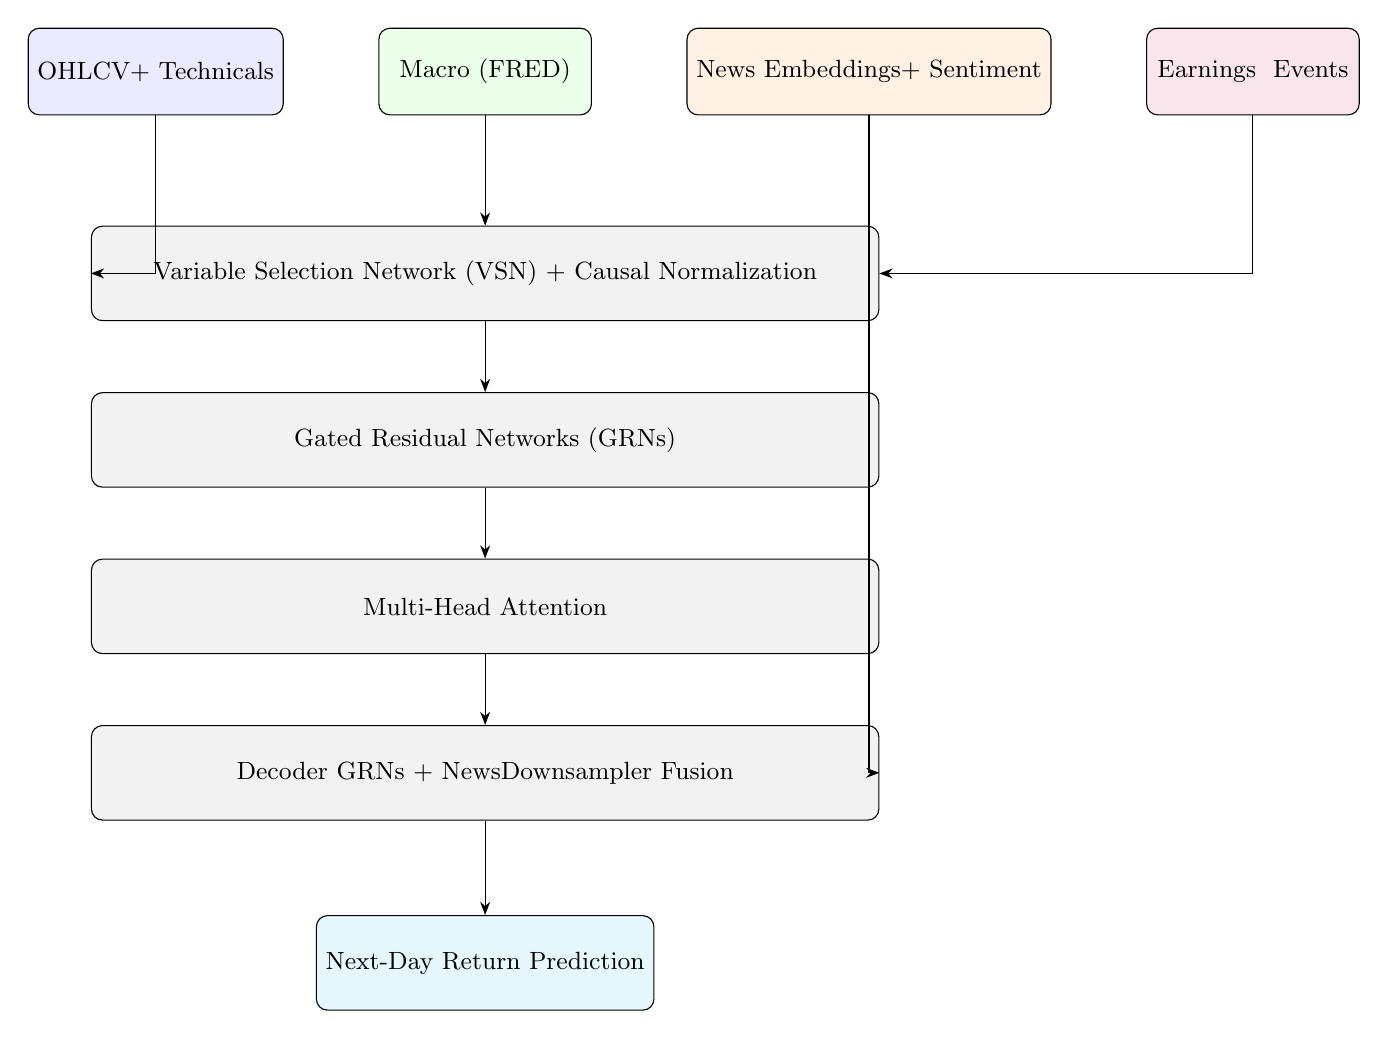
\begin{tikzpicture}[node distance=8mm and 12mm, every node/.style={font=\small}]
    % Inputs
    \node[draw, rounded corners, fill=blue!8, minimum width=2.9cm, minimum height=1.1cm] (ohlc) {OHLCV\\+ Technicals};
    \node[draw, rounded corners, fill=green!8, right=of ohlc, minimum width=2.7cm, minimum height=1.1cm] (macro) {Macro (FRED)};
    \node[draw, rounded corners, fill=orange!10, right=of macro, minimum width=2.7cm, minimum height=1.1cm] (news) {News Embeddings\\+ Sentiment};
    \node[draw, rounded corners, fill=purple!10, right=of news, minimum width=2.7cm, minimum height=1.1cm] (events) {Earnings \/ Events};

    % Fusion
    \node[draw, rounded corners, fill=gray!10, below=14mm of macro, minimum width=10cm, minimum height=1.2cm] (vsn) {Variable Selection Network (VSN) + Causal Normalization};

    % Encoder / Attention / Decoder
    \node[draw, rounded corners, fill=gray!10, below=9mm of vsn, minimum width=10cm, minimum height=1.2cm] (grn) {Gated Residual Networks (GRNs)};
    \node[draw, rounded corners, fill=gray!10, below=9mm of grn, minimum width=10cm, minimum height=1.2cm] (attn) {Multi-Head Attention};
    \node[draw, rounded corners, fill=gray!10, below=9mm of attn, minimum width=10cm, minimum height=1.2cm] (dec) {Decoder GRNs + NewsDownsampler Fusion};

    % Output
    \node[draw, rounded corners, fill=cyan!10, below=12mm of dec, minimum width=4.2cm, minimum height=1.2cm] (pred) {Next-Day Return Prediction};

    % Arrows
    \draw[-{Stealth}] (ohlc.south) |- (vsn.west);
    \draw[-{Stealth}] (macro.south) -- (vsn.north);
    \draw[-{Stealth}] (events.south) |- (vsn.east);
    \draw[-{Stealth}] (news.south) |- (dec.east);
    \draw[-{Stealth}] (vsn) -- (grn);
    \draw[-{Stealth}] (grn) -- (attn);
    \draw[-{Stealth}] (attn) -- (dec);
    \draw[-{Stealth}] (dec) -- (pred);
  \end{tikzpicture}
  \caption{TFT-based multi-modal forecasting pipeline implemented in the repository.}
\end{figure}

\subsection{Experimental Configuration}
We adopt daily frequency, encoder windows of 30--60 days, and one-step-ahead targets. Training uses AdamW with cosine annealing and gradient clipping. For honest validation, we use temporal splits with a 21-day gap and optional symbol holdout; validation loaders reuse training scalers to avoid leakage. All settings are configurable in \texttt{unified\_tft\_pipeline.py}.

\subsection{Ablation Design}
We vary both \emph{modalities} and \emph{model families}:
\begin{itemize}[leftmargin=*]
  \item Modalities: Full (OHLCV + technical + macro + news + events), \emph{No economic}, \emph{No news}, \emph{No technical}, and \emph{Only OHLCV}.
  \item Models: Ridge, Random Forest, XGBoost, LSTM-based RNNs, and TFT/Enhanced-TFT.
\end{itemize}
Metrics include MSE, MAE, R$^2$, MAPE; trend metrics (directional accuracy, ROC-AUC); and finance metrics (annualized return of predicted path, Sharpe, and maximum drawdown). The trading simulator reports strategy vs benchmarks (DCA, buy-and-hold) and win rates.

\subsection{Representative Results}
Figure~\ref{fig:aapl-ablation} summarizes a representative single-stock ablation (AAPL). Where images are unavailable locally, a placeholder is rendered. Directional accuracy across models clustered near 0.53--0.59, with TFT not consistently surpassing LSTM baselines on daily horizons. R$^2$ on raw returns is typically near zero or negative, reflecting the well-known difficulty of point-return regression at daily cadence. Sharpe improvements appear for tree models under certain feature subsets, highlighting the value of nonparametric ensembles when signals are sparse.

\begin{figure}[H]
  \centering
  % Place your image at figures/aapl_ablation_heatmap.png to auto-include.
  \IfFileExists{figures/aapl_ablation_heatmap.png}{%
    \includegraphics[width=0.98\textwidth]{figures/aapl_ablation_heatmap.png}%
  }{%
    \fbox{\parbox{0.95\textwidth}{\centering Placeholder for AAPL Ablation Heatmap\\(copy your figure to figures/aapl\_ablation\_heatmap.png)}}%
  }
  \caption{Ablation study heatmaps (R$^2$, directional accuracy, Sharpe) for AAPL across models and feature subsets.}
  \label{fig:aapl-ablation}
\end{figure}

\subsection{Findings}
\begin{itemize}[leftmargin=*]
  \item \textbf{Model capacity vs data regime}: RNNs often outperformed TFT on daily single-step returns, likely due to fewer parameters and better bias--variance trade-offs in low SNR conditions.
  \item \textbf{News impact}: News embeddings and sentiment aided specific market regimes but did not universally improve directional accuracy; their benefit increased when combined with robust normalization and longer context.
  \item \textbf{Macro features}: Select macro time series improved stability and Sharpe by moderating exposure during risk-off regimes.
  \item \textbf{Interpretability}: VSN weights and attention maps identified periods where technicals dominated vs. news/economic drivers, consistent with feature-group summaries produced by the pipeline.
\end{itemize}

\subsection{Portfolio Simulation}
We evaluated utility via the included \texttt{TradingSimulator}, producing equity curves and summary reports (Sharpe, max drawdown, profit factor, and trade counts). Benchmarks include DCA and buy-and-hold. Example outputs in the repository demonstrate realistic, conservative performance expectations (e.g., modest Sharpe and sometimes underperformance to buy-and-hold)—a desired trait when leakage is eliminated and costs are not ignored.

\subsection{Reproducibility}
All experiments are reproducible with CLI commands such as:
\begin{verbatim}
python Hayson/TFT/unified_tft_pipeline.py --epochs 5 --symbols AAPL,MSFT
python Hayson/TFT/unified_tft_pipeline.py --out-of-sample temporal --temporal-split 0.8
\end{verbatim}
Key code locations: data loaders and caching (\texttt{Hayson/TFT/dataModule}), TFT model (\texttt{tft\_multimodal.py}), training and analysis (\texttt{unified\_tft\_pipeline.py}).

%------------------------------------------------------------------------------
% Initiative II – Krackle
%------------------------------------------------------------------------------
\section{Initiative II: Krackle – Real-Time Smile Detection Web Game}
\subsection{Motivation}
Krackle explores affective computing in the browser: players trigger events by smiling, testing latency, robustness, and privacy of on-device CV.

\subsection{System Architecture}
\begin{figure}[H]
  \centering
  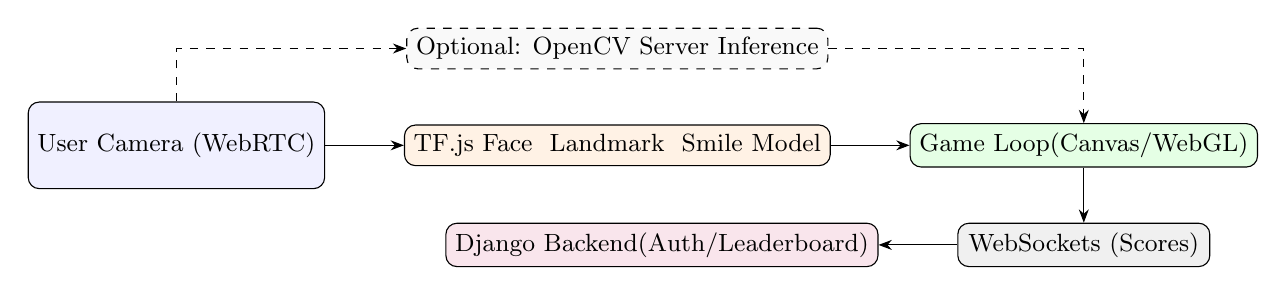
\begin{tikzpicture}[node distance=7mm and 10mm, every node/.style={font=\small}]
    \node[draw, rounded corners, fill=blue!6, minimum width=3.2cm, minimum height=1.1cm] (cam) {User Camera (WebRTC)};
    \node[draw, rounded corners, fill=orange!10, right=of cam, minimum width=3.6cm] (tfjs) {TF.js Face \/ Landmark \/ Smile Model};
    \node[draw, rounded corners, fill=green!10, right=of tfjs, minimum width=3cm] (game) {Game Loop \\ (Canvas/WebGL)};
    \node[draw, rounded corners, fill=gray!12, below=of game, minimum width=3.2cm] (ws) {WebSockets (Scores)};
    \node[draw, rounded corners, fill=purple!10, left=of ws, minimum width=3.4cm] (django) {Django Backend \\ (Auth/Leaderboard)};
    \node[draw, dashed, rounded corners, fill=gray!5, above=of tfjs, minimum width=5.2cm] (opencv) {Optional: OpenCV Server Inference};
    \draw[-{Stealth}] (cam) -- (tfjs);
    \draw[-{Stealth}] (tfjs) -- (game);
    \draw[-{Stealth}] (game) -- (ws);
    \draw[-{Stealth}] (ws) -- (django);
    \draw[-{Stealth}, dashed] (cam) |- (opencv);
    \draw[-{Stealth}, dashed] (opencv) -| (game);
  \end{tikzpicture}
  \caption{Krackle architecture: on-device TF.js inference, real-time game loop, and optional server-side fallback.}
\end{figure}

\subsection{Technology Stack}
\begin{itemize}[leftmargin=*]
  \item \textbf{Front-end}: JavaScript/TypeScript, WebGL, Canvas, TensorFlow.js models (MobileNet/MediaPipe/BlazeFace variants).
  \item \textbf{Back-end}: Django (REST + templates), Channels (WebSockets) for live leaderboards; Redis for pub/sub.
  \item \textbf{Computer Vision}: TF.js for on-device; Python OpenCV + dlib as optional server fallback (GPU if available).
\end{itemize}

\subsection{Face/Emotion Detection and Gameplay}
Face boxes and landmarks are detected each frame; a smile score (mouth aspect ratio + classifier logit) triggers in-game events. Smoothing and hysteresis avoid flicker. The game awards points for sustained smiles, supports difficulty curves, and debounces over-sensitivity.

\subsection{Privacy and Ethics}
Default mode performs \emph{on-device} inference; raw frames never leave the browser. Only anonymized events (e.g., \texttt{"smile:on"}) and scores transit via WebSockets. Explicit consent dialogs describe data flow; no biometric templates are stored server-side. An accessibility mode permits keyboard-controlled play.

\subsection{Deliverables}
Working prototype, documentation, and demo instructions; optional public leaderboard can be disabled for private sessions.

%------------------------------------------------------------------------------
% Lessons, Limitations, and Future Work
%------------------------------------------------------------------------------
\section{Lessons Learned}
\begin{itemize}[leftmargin=*]
  \item Prevention of leakage (temporal gaps, shared scalers, symbol holdout) is essential; honest metrics are typically lower but credible.
  \item Daily single-step returns are extremely noisy; classification of direction and risk-aware backtesting convey more utility than raw MSE.
  \item On-device CV with TF.js provides excellent UX and privacy; careful thresholding and smoothing are key to robustness.
\end{itemize}

\section{Limitations and Future Work}
\begin{itemize}[leftmargin=*]
  \item Explore multi-horizon targets (1, 5, 10 days) and regime-aware training for TFT; consider contrastive pretraining for news embeddings.
  \item Incorporate transaction costs and slippage in the trading simulator; expand to portfolio-level optimization and risk parity.
  \item For Krackle, add federated learning for on-device personalization and evaluate differential privacy for telemetry.
\end{itemize}

\section{Conclusion}
This internship delivered a robust research platform for multi-modal stock prediction and a novel real-time affective game. Empirical studies underscored that, under strict leakage controls, simpler sequence models (LSTMs) can outperform transformers on daily returns, while certain feature subsets (technicals, selective macro) improve risk-adjusted performance. Krackle demonstrated the feasibility of privacy-preserving, low-latency smile-driven interactions on the web.

%------------------------------------------------------------------------------
% References (examples – extend as needed)
%------------------------------------------------------------------------------
\section*{References}
\begin{itemize}
  \item Lim, B., et al. (2021). Temporal Fusion Transformers for Interpretable Multi-horizon Time Series Forecasting.
  \item Vaswani, A., et al. (2017). Attention Is All You Need.
  \item Repository documentation: \href{\repoLink}{\repoLink}
\end{itemize}

%------------------------------------------------------------------------------
% Appendices (pull in existing .tex if present)
%------------------------------------------------------------------------------
\appendix
\section{Implementation Roadmap}
\IfFileExists{implementation_roadmap.tex}{\documentclass[11pt]{article}
\usepackage[utf8]{inputenc}
\usepackage[T1]{fontenc}
\usepackage{geometry}
\usepackage{xcolor}
\usepackage{booktabs}
\usepackage{array}
\usepackage{enumitem}
\usepackage{amsmath}
\usepackage{amssymb}
\usepackage{hyperref}
\usepackage{listings}
\usepackage{fancyvrb}

\geometry{margin=1in}

% Custom colors
\definecolor{codeblue}{RGB}{0, 102, 204}
\definecolor{codegray}{RGB}{128, 128, 128}
\definecolor{codegreen}{RGB}{0, 128, 0}
\definecolor{codepurple}{RGB}{128, 0, 128}

% Code styling
\lstdefinestyle{pythonstyle}{
    language=Python,
    basicstyle=\ttfamily\footnotesize,
    keywordstyle=\color{codeblue},
    commentstyle=\color{codegreen},
    stringstyle=\color{codepurple},
    numberstyle=\tiny\color{codegray},
    breaklines=true,
    captionpos=b,
    frame=single,
    numbers=left,
    showstringspaces=false
}

\title{\textbf{Multi-Modal Stock TFT Implementation Roadmap} \\ 
       \large{Detailed Technical Specifications and Code Structure}}
\author{Implementation Guide - August 2025}
\date{}

\begin{document}

\maketitle

\section{Current Codebase Analysis}

Based on the existing codebase analysis, the project has a solid foundation with the following components already implemented:

\subsection{Existing Infrastructure}
\begin{itemize}
    \item ✅ \textbf{TFT Core:} Production-ready TFT implementation in \texttt{tft\_multimodal.py}
    \item ✅ \textbf{Data Pipeline:} Robust multimodal data loading via \texttt{dataModule/}
    \item ✅ \textbf{Training:} Unified training pipeline in \texttt{unified\_tft\_pipeline.py}
    \item ✅ \textbf{Trading Simulation:} Kelly criterion, DCA strategies in \texttt{trading\_simulator.py}
    \item ✅ \textbf{Visualization:} OHLC plotting with predictions in \texttt{ohlc\_plotter.py}
    \item ✅ \textbf{Caching:} Intelligent data caching system
    \item ⚠️ \textbf{Baselines:} Partial implementation in \texttt{fixed\_baseline\_pipeline.py}
\end{itemize}

\subsection{Current Baseline Models}
\begin{itemize}
    \item ✅ Linear Regression
    \item ✅ Random Forest Regressor
    \item ✅ XGBoost (optional, if installed)
    \item ❌ LSTM variants
    \item ❌ Transformer baselines
    \item ❌ Financial time series models
    \item ❌ Deep learning ensemble methods
\end{itemize}

\section{Implementation Tasks by Priority}

\subsection{Priority 1: Complete Baseline Suite (Days 1-7)}

\subsubsection{Task 1.1: Extend \texttt{fixed\_baseline\_pipeline.py}}

Add the following model implementations to the existing baseline runner:

\begin{lstlisting}[style=pythonstyle, caption=Enhanced Baseline Models]
# Add to fixed_baseline_pipeline.py after line 398

# LSTM-based models
from tensorflow.keras.models import Sequential
from tensorflow.keras.layers import LSTM, Dense, Dropout, Bidirectional

class LSTMWrapper:
    """Keras LSTM wrapper for sklearn-like interface"""
    def __init__(self, sequence_length=60, units=50, layers=2):
        self.sequence_length = sequence_length
        self.units = units
        self.layers = layers
        self.model = None
        
    def fit(self, X, y):
        # Reshape X for LSTM: (samples, timesteps, features)
        X_lstm = X.reshape(-1, self.sequence_length, X.shape[1]//self.sequence_length)
        
        self.model = Sequential()
        self.model.add(LSTM(self.units, return_sequences=True, 
                           input_shape=(self.sequence_length, X.shape[1]//self.sequence_length)))
        self.model.add(Dropout(0.2))
        
        for _ in range(self.layers - 1):
            self.model.add(LSTM(self.units, return_sequences=True))
            self.model.add(Dropout(0.2))
            
        self.model.add(LSTM(self.units))
        self.model.add(Dropout(0.2))
        self.model.add(Dense(y.shape[1] if len(y.shape) > 1 else 1))
        
        self.model.compile(optimizer='adam', loss='mse')
        self.model.fit(X_lstm, y, epochs=50, batch_size=32, verbose=0)
        
    def predict(self, X):
        X_lstm = X.reshape(-1, self.sequence_length, X.shape[1]//self.sequence_length)
        return self.model.predict(X_lstm, verbose=0)

# Add ARIMA models
from statsmodels.tsa.arima.model import ARIMA
from statsmodels.tsa.statespace.sarimax import SARIMAX

class ARIMAWrapper:
    """ARIMA wrapper for multivariate prediction"""
    def __init__(self, order=(1,1,1)):
        self.order = order
        self.models = []
        
    def fit(self, X, y):
        self.models = []
        for i in range(y.shape[1] if len(y.shape) > 1 else 1):
            target = y[:, i] if len(y.shape) > 1 else y
            model = ARIMA(target, order=self.order)
            fitted_model = model.fit()
            self.models.append(fitted_model)
            
    def predict(self, X):
        predictions = []
        for model in self.models:
            pred = model.forecast(steps=1)
            predictions.append(pred[0] if hasattr(pred, '__len__') else pred)
        return np.array(predictions).reshape(1, -1)

# Update the base_models dictionary
enhanced_models = {
    'LSTM_Vanilla': LSTMWrapper(units=50, layers=1),
    'LSTM_Deep': LSTMWrapper(units=100, layers=3),
    'LSTM_Bidirectional': None,  # Implement separately
    'ARIMA': ARIMAWrapper(order=(2,1,2)),
    'SARIMAX': None,  # Seasonal ARIMA
}
\end{lstlisting}

\subsubsection{Task 1.2: Create Advanced Ensemble Methods}

Create \texttt{ensemble\_baselines.py}:

\begin{lstlisting}[style=pythonstyle, caption=Ensemble Baseline Methods]
#!/usr/bin/env python3
"""
Advanced Ensemble Methods for Stock Prediction Baselines
========================================================
"""

import numpy as np
from sklearn.ensemble import VotingRegressor, StackingRegressor
from sklearn.model_selection import cross_val_score
from sklearn.metrics import mean_squared_error

class AdaptiveEnsemble:
    """Dynamically weighted ensemble based on recent performance"""
    
    def __init__(self, base_models, window_size=252):  # 1 trading year
        self.base_models = base_models
        self.window_size = window_size
        self.weights = None
        self.performance_history = []
        
    def fit(self, X, y):
        # Train all base models
        for name, model in self.base_models.items():
            model.fit(X, y)
            
        # Initialize equal weights
        self.weights = {name: 1.0/len(self.base_models) 
                       for name in self.base_models.keys()}
                       
    def predict(self, X):
        predictions = {}
        for name, model in self.base_models.items():
            predictions[name] = model.predict(X)
            
        # Weighted average prediction
        final_pred = np.zeros_like(list(predictions.values())[0])
        for name, pred in predictions.items():
            final_pred += self.weights[name] * pred
            
        return final_pred
        
    def update_weights(self, y_true, predictions):
        """Update weights based on recent performance"""
        errors = {}
        for name, pred in predictions.items():
            errors[name] = mean_squared_error(y_true, pred)
            
        # Inverse error weighting
        total_inv_error = sum(1.0/error for error in errors.values())
        for name in self.weights.keys():
            self.weights[name] = (1.0/errors[name]) / total_inv_error

class MetaLearningEnsemble:
    """Meta-learning ensemble using model predictions as features"""
    
    def __init__(self, base_models, meta_model):
        self.base_models = base_models
        self.meta_model = meta_model
        
    def fit(self, X, y):
        # Train base models with cross-validation to get meta-features
        meta_features = []
        
        for name, model in self.base_models.items():
            # Cross-validation predictions as meta-features
            cv_predictions = cross_val_score(model, X, y, cv=5, 
                                           scoring='neg_mean_squared_error')
            meta_features.append(cv_predictions)
            
            # Train on full dataset
            model.fit(X, y)
            
        meta_X = np.column_stack(meta_features)
        self.meta_model.fit(meta_X, y)
        
    def predict(self, X):
        # Get base model predictions
        base_predictions = []
        for name, model in self.base_models.items():
            pred = model.predict(X)
            base_predictions.append(pred.flatten())
            
        meta_X = np.column_stack(base_predictions)
        return self.meta_model.predict(meta_X)
\end{lstlisting}

\subsection{Priority 2: Multi-Asset Evaluation Framework (Days 8-21)}

\subsubsection{Task 2.1: Create Stock Grouping System}

Create \texttt{stock\_groups.py}:

\begin{lstlisting}[style=pythonstyle, caption=Stock Categorization System]
#!/usr/bin/env python3
"""
Stock Grouping and Sector Analysis
==================================
"""

STOCK_GROUPS = {
    'technology': {
        'symbols': ['AAPL', 'MSFT', 'GOOGL', 'NVDA', 'AMZN', 'TSLA', 'META', 'NFLX'],
        'description': 'Large-cap technology stocks',
        'characteristics': ['High volatility', 'Growth-oriented', 'Innovation-driven']
    },
    'financial': {
        'symbols': ['JPM', 'BAC', 'WFC', 'GS', 'MS', 'C', 'BRK-B'],
        'description': 'Major financial institutions',
        'characteristics': ['Interest rate sensitive', 'Economic cycle dependent']
    },
    'healthcare': {
        'symbols': ['JNJ', 'PFE', 'UNH', 'MRCK', 'ABBV', 'TMO', 'DHR'],
        'description': 'Healthcare and pharmaceutical companies',
        'characteristics': ['Defensive', 'Regulatory sensitive', 'Stable cash flows']
    },
    'consumer_discretionary': {
        'symbols': ['AMZN', 'TSLA', 'HD', 'MCD', 'NKE', 'SBUX', 'DIS'],
        'description': 'Consumer discretionary companies',
        'characteristics': ['Economic cycle sensitive', 'Consumer spending dependent']
    },
    'consumer_staples': {
        'symbols': ['KO', 'PEP', 'WMT', 'PG', 'JNJ', 'PFE'],
        'description': 'Consumer staples and essentials',
        'characteristics': ['Defensive', 'Stable demand', 'Dividend-focused']
    },
    'energy': {
        'symbols': ['XOM', 'CVX', 'COP', 'EOG', 'SLB', 'MPC'],
        'description': 'Energy sector companies',
        'characteristics': ['Commodity sensitive', 'Cyclical', 'High volatility']
    },
    'indices': {
        'symbols': ['SPY', 'QQQ', 'DIA', 'IWM', 'VTI'],
        'description': 'Major market indices ETFs',
        'characteristics': ['Diversified', 'Market representative', 'Lower volatility']
    }
}

MARKET_CONDITIONS = {
    'bull_market_2020_2021': {
        'start_date': '2020-03-23',
        'end_date': '2021-11-05',
        'description': 'COVID recovery bull market',
        'characteristics': ['Low interest rates', 'Fiscal stimulus', 'Tech outperformance']
    },
    'bear_market_2022': {
        'start_date': '2022-01-01',
        'end_date': '2022-10-12',
        'description': 'Inflation and rate hike bear market',
        'characteristics': ['Rising rates', 'Inflation concerns', 'Value outperformance']
    },
    'volatile_2023': {
        'start_date': '2023-01-01',
        'end_date': '2023-12-31',
        'description': 'Banking crisis and AI boom volatility',
        'characteristics': ['Banking stress', 'AI hype', 'Selective outperformance']
    }
}

def get_comparison_pairs():
    """Return meaningful stock comparison pairs for analysis"""
    return [
        ('AAPL', 'MSFT'),      # Tech giants
        ('JPM', 'BAC'),        # Major banks
        ('KO', 'PEP'),         # Beverage rivals
        ('SPY', 'QQQ'),        # Broad vs tech-heavy market
        ('XOM', 'CVX'),        # Energy majors
    ]

def get_sector_representatives():
    """Return one representative stock per major sector"""
    return {
        'Technology': 'AAPL',
        'Financial': 'JPM', 
        'Healthcare': 'JNJ',
        'Consumer Discretionary': 'AMZN',
        'Consumer Staples': 'KO',
        'Energy': 'XOM',
        'Market Index': 'SPY'
    }
\end{lstlisting}

\subsubsection{Task 2.2: Create Comprehensive Evaluation Runner}

Create \texttt{comprehensive\_evaluation.py}:

\begin{lstlisting}[style=pythonstyle, caption=Multi-Asset Evaluation Framework]
#!/usr/bin/env python3
"""
Comprehensive Multi-Asset Evaluation Framework
=============================================
"""

import pandas as pd
import numpy as np
from typing import Dict, List, Tuple
from concurrent.futures import ThreadPoolExecutor, as_completed
import logging
from stock_groups import STOCK_GROUPS, MARKET_CONDITIONS

class ComprehensiveEvaluator:
    """Runs systematic evaluation across multiple assets and conditions"""
    
    def __init__(self, models: Dict, config: Dict):
        self.models = models
        self.config = config
        self.results = {}
        
    def run_full_evaluation(self):
        """Run complete evaluation across all stocks and conditions"""
        
        # 1. Individual stock evaluation
        self.evaluate_by_stock_groups()
        
        # 2. Market condition analysis
        self.evaluate_by_market_conditions()
        
        # 3. Cross-sectional analysis
        self.evaluate_cross_sectional()
        
        # 4. Pair trading analysis
        self.evaluate_pair_trading()
        
        return self.results
        
    def evaluate_by_stock_groups(self):
        """Evaluate models performance by stock sector/group"""
        
        for group_name, group_info in STOCK_GROUPS.items():
            print(f"\\n📊 Evaluating {group_name.upper()} sector...")
            
            group_results = {}
            symbols = group_info['symbols']
            
            # Parallel evaluation of stocks in group
            with ThreadPoolExecutor(max_workers=4) as executor:
                future_to_symbol = {
                    executor.submit(self.evaluate_single_stock, symbol): symbol 
                    for symbol in symbols
                }
                
                for future in as_completed(future_to_symbol):
                    symbol = future_to_symbol[future]
                    try:
                        result = future.result()
                        group_results[symbol] = result
                    except Exception as exc:
                        print(f'❌ {symbol} generated exception: {exc}')
                        
            self.results[f'group_{group_name}'] = group_results
            
    def evaluate_by_market_conditions(self):
        """Evaluate model performance under different market conditions"""
        
        for condition_name, condition_info in MARKET_CONDITIONS.items():
            print(f"\\n📈 Evaluating {condition_name} period...")
            
            # Filter data by date range
            start_date = condition_info['start_date']
            end_date = condition_info['end_date']
            
            condition_results = {}
            
            # Test representative stocks in this period
            test_symbols = ['AAPL', 'JPM', 'SPY']  # Representative cross-section
            
            for symbol in test_symbols:
                result = self.evaluate_single_stock(
                    symbol, 
                    start_date=start_date, 
                    end_date=end_date
                )
                condition_results[symbol] = result
                
            self.results[f'condition_{condition_name}'] = condition_results
            
    def evaluate_single_stock(self, symbol: str, start_date=None, end_date=None):
        """Evaluate all models on a single stock"""
        
        # Load data for symbol with date filters
        data_loader = self.get_data_loader(symbol, start_date, end_date)
        X_train, y_train, X_test, y_test = data_loader.get_train_test_split()
        
        stock_results = {}
        
        for model_name, model in self.models.items():
            try:
                # Train model
                model.fit(X_train, y_train)
                
                # Generate predictions
                y_pred = model.predict(X_test)
                
                # Calculate metrics
                metrics = self.calculate_metrics(y_test, y_pred)
                
                # Calculate trading performance
                trading_metrics = self.calculate_trading_metrics(
                    y_test, y_pred, symbol
                )
                
                stock_results[model_name] = {
                    'prediction_metrics': metrics,
                    'trading_metrics': trading_metrics
                }
                
            except Exception as e:
                print(f"❌ Error with {model_name} on {symbol}: {e}")
                stock_results[model_name] = {'error': str(e)}
                
        return stock_results
\end{lstlisting}

\subsection{Priority 3: Statistical Analysis Framework (Days 22-28)}

\subsubsection{Task 3.1: Create Statistical Testing Suite}

Create \texttt{statistical\_analysis.py}:

\begin{lstlisting}[style=pythonstyle, caption=Statistical Analysis Framework]
#!/usr/bin/env python3
"""
Statistical Analysis and Significance Testing
=============================================
"""

import numpy as np
import pandas as pd
from scipy import stats
from scipy.stats import friedmanchisquare
import scikit_posthocs as sp
from typing import Dict, List, Tuple

class StatisticalAnalyzer:
    """Comprehensive statistical analysis of model performance"""
    
    def __init__(self, results: Dict):
        self.results = results
        self.analysis_results = {}
        
    def run_full_analysis(self):
        """Run complete statistical analysis"""
        
        # 1. Descriptive statistics
        self.calculate_descriptive_stats()
        
        # 2. Significance testing
        self.run_significance_tests()
        
        # 3. Effect size analysis
        self.calculate_effect_sizes()
        
        # 4. Risk analysis
        self.analyze_risk_metrics()
        
        return self.analysis_results
        
    def calculate_descriptive_stats(self):
        """Calculate descriptive statistics for all models"""
        
        model_performance = self.aggregate_model_performance()
        
        desc_stats = {}
        for metric in ['mse', 'mae', 'sharpe_ratio', 'max_drawdown']:
            desc_stats[metric] = {}
            
            for model_name in model_performance.keys():
                values = model_performance[model_name][metric]
                
                desc_stats[metric][model_name] = {
                    'mean': np.mean(values),
                    'std': np.std(values),
                    'median': np.median(values),
                    'q25': np.percentile(values, 25),
                    'q75': np.percentile(values, 75),
                    'min': np.min(values),
                    'max': np.max(values)
                }
                
        self.analysis_results['descriptive_stats'] = desc_stats
        
    def run_significance_tests(self):
        """Run statistical significance tests comparing models"""
        
        model_performance = self.aggregate_model_performance()
        significance_results = {}
        
        for metric in ['mse', 'mae', 'sharpe_ratio']:
            print(f"\\n🧮 Testing significance for {metric}...")
            
            # Prepare data for Friedman test
            model_names = list(model_performance.keys())
            data_matrix = []
            
            for model_name in model_names:
                data_matrix.append(model_performance[model_name][metric])
                
            # Friedman test (non-parametric ANOVA for repeated measures)
            statistic, p_value = friedmanchisquare(*data_matrix)
            
            significance_results[metric] = {
                'friedman_statistic': statistic,
                'p_value': p_value,
                'significant': p_value < 0.05
            }
            
            # Post-hoc analysis if significant
            if p_value < 0.05:
                df = pd.DataFrame(data_matrix, index=model_names).T
                posthoc = sp.posthoc_nemenyi_friedman(df)
                significance_results[metric]['posthoc'] = posthoc
                
        self.analysis_results['significance_tests'] = significance_results
        
    def calculate_effect_sizes(self):
        """Calculate effect sizes for model comparisons"""
        
        model_performance = self.aggregate_model_performance()
        effect_sizes = {}
        
        # Cohen's d for pairwise comparisons
        model_names = list(model_performance.keys())
        
        for metric in ['mse', 'mae', 'sharpe_ratio']:
            effect_sizes[metric] = {}
            
            for i, model1 in enumerate(model_names):
                for j, model2 in enumerate(model_names[i+1:], i+1):
                    
                    values1 = model_performance[model1][metric]
                    values2 = model_performance[model2][metric]
                    
                    # Cohen's d
                    pooled_std = np.sqrt(((len(values1)-1)*np.var(values1) + 
                                        (len(values2)-1)*np.var(values2)) / 
                                       (len(values1) + len(values2) - 2))
                    
                    cohens_d = (np.mean(values1) - np.mean(values2)) / pooled_std
                    
                    effect_sizes[metric][f'{model1}_vs_{model2}'] = {
                        'cohens_d': cohens_d,
                        'magnitude': self.interpret_cohens_d(cohens_d)
                    }
                    
        self.analysis_results['effect_sizes'] = effect_sizes
        
    @staticmethod
    def interpret_cohens_d(d):
        """Interpret Cohen's d effect size"""
        abs_d = abs(d)
        if abs_d < 0.2:
            return 'negligible'
        elif abs_d < 0.5:
            return 'small'
        elif abs_d < 0.8:
            return 'medium'
        else:
            return 'large'
\end{lstlisting}

\subsection{Priority 4: Paper Generation Framework (Days 26-31)}

\subsubsection{Task 4.1: Automated Results Table Generation}

Create \texttt{paper\_generator.py}:

\begin{lstlisting}[style=pythonstyle, caption=Automated Paper Generation]
#!/usr/bin/env python3
"""
Automated Research Paper Content Generation
===========================================
"""

import pandas as pd
import matplotlib.pyplot as plt
import seaborn as sns
from typing import Dict, Any

class PaperGenerator:
    """Generate LaTeX tables and figures for research paper"""
    
    def __init__(self, results: Dict, analysis: Dict):
        self.results = results
        self.analysis = analysis
        
    def generate_main_results_table(self):
        """Generate main results comparison table"""
        
        latex_table = r"""
\\begin{table}[htbp]
\\centering
\\caption{Model Performance Comparison Across All Stocks}
\\label{tab:main_results}
\\begin{tabular}{lcccccc}
\\toprule
Model & MAE & RMSE & Dir. Acc. & Sharpe & Max DD & Win Rate \\\\
\\midrule
"""
        
        # Extract aggregated results
        for model_name in self.get_model_names():
            metrics = self.get_aggregated_metrics(model_name)
            
            latex_table += f"{model_name} & "
            latex_table += f"{metrics['mae']:.4f} & "
            latex_table += f"{metrics['rmse']:.4f} & "
            latex_table += f"{metrics['directional_accuracy']:.3f} & "
            latex_table += f"{metrics['sharpe_ratio']:.3f} & "
            latex_table += f"{metrics['max_drawdown']:.3f} & "
            latex_table += f"{metrics['win_rate']:.3f} \\\\\\\\"
            
        latex_table += r"""
\\bottomrule
\\end{tabular}
\\end{table}
"""
        
        return latex_table
        
    def generate_sector_analysis_table(self):
        """Generate sector-wise performance analysis"""
        
        latex_table = r"""
\\begin{table}[htbp]
\\centering
\\caption{TFT Performance by Market Sector}
\\label{tab:sector_analysis}
\\begin{tabular}{lccccc}
\\toprule
Sector & Sharpe Ratio & Max Drawdown & Total Return & Volatility & \\# Stocks \\\\
\\midrule
"""
        
        for sector in ['Technology', 'Financial', 'Healthcare', 'Consumer', 'Energy']:
            sector_metrics = self.get_sector_metrics(sector)
            
            latex_table += f"{sector} & "
            latex_table += f"{sector_metrics['sharpe_ratio']:.3f} & "
            latex_table += f"{sector_metrics['max_drawdown']:.3f} & "
            latex_table += f"{sector_metrics['total_return']:.3f} & "
            latex_table += f"{sector_metrics['volatility']:.3f} & "
            latex_table += f"{sector_metrics['num_stocks']} \\\\\\\\"
            
        latex_table += r"""
\\bottomrule
\\end{tabular}
\\end{table}
"""
        
        return latex_table
        
    def generate_significance_table(self):
        """Generate statistical significance results table"""
        
        significance = self.analysis['significance_tests']
        
        latex_table = r"""
\\begin{table}[htbp]
\\centering
\\caption{Statistical Significance Tests (Friedman Test)}
\\label{tab:significance}
\\begin{tabular}{lccc}
\\toprule
Metric & Test Statistic & p-value & Significant \\\\
\\midrule
"""
        
        for metric, results in significance.items():
            latex_table += f"{metric.upper()} & "
            latex_table += f"{results['friedman_statistic']:.3f} & "
            latex_table += f"{results['p_value']:.4f} & "
            latex_table += f"{'Yes' if results['significant'] else 'No'} \\\\\\\\"
            
        latex_table += r"""
\\bottomrule
\\end{tabular}
\\end{table}
"""
        
        return latex_table
        
    def generate_all_tables(self):
        """Generate all tables for the paper"""
        
        tables = {
            'main_results': self.generate_main_results_table(),
            'sector_analysis': self.generate_sector_analysis_table(),
            'significance': self.generate_significance_table()
        }
        
        return tables
\end{lstlisting}

\section{Daily Task Breakdown}

\subsection{Week 1: Baseline Implementation}

\textbf{Day 1-2:} LSTM and Deep Learning Baselines
\begin{itemize}
    \item Implement LSTM variants (vanilla, bidirectional, stacked)
    \item Add GRU models and CNN-LSTM hybrid
    \item Integrate with existing \texttt{fixed\_baseline\_pipeline.py}
\end{itemize}

\textbf{Day 3-4:} Traditional ML Enhancement
\begin{itemize}
    \item Add LightGBM, CatBoost, Extra Trees
    \item Implement SVM with different kernels
    \item Add ensemble methods (voting, stacking)
\end{itemize}

\textbf{Day 5-6:} Financial Time Series Models
\begin{itemize}
    \item Implement ARIMA, GARCH, VAR models
    \item Add Markov switching models
    \item Create naive baselines (random walk, moving averages)
\end{itemize}

\textbf{Day 7:} Testing and Integration
\begin{itemize}
    \item Test all baseline models
    \item Fix integration issues
    \item Validate output consistency
\end{itemize}

\subsection{Week 2-3: Multi-Asset Evaluation}

\textbf{Day 8-10:} Stock Group Analysis
\begin{itemize}
    \item Implement \texttt{stock\_groups.py}
    \item Run technology sector analysis
    \item Run financial sector analysis
\end{itemize}

\textbf{Day 11-14:} Comprehensive Stock Coverage
\begin{itemize}
    \item Healthcare and consumer sectors
    \item Energy and utilities sectors
    \item Index ETF analysis
\end{itemize}

\textbf{Day 15-17:} Market Condition Analysis
\begin{itemize}
    \item Bull market periods (2020-2021)
    \item Bear market periods (2022)
    \item Volatile periods (2023-2024)
\end{itemize}

\textbf{Day 18-21:} Cross-sectional Analysis
\begin{itemize}
    \item Pair trading analysis
    \item Correlation studies
    \item Portfolio-level evaluation
\end{itemize}

\subsection{Week 4: Statistical Analysis}

\textbf{Day 22-24:} Core Statistical Testing
\begin{itemize}
    \item Implement \texttt{statistical\_analysis.py}
    \item Run Friedman tests for model comparison
    \item Calculate effect sizes (Cohen's d)
\end{itemize}

\textbf{Day 25-26:} Advanced Analytics
\begin{itemize}
    \item Risk-adjusted performance metrics
    \item Regime-dependent analysis
    \item Robustness testing
\end{itemize}

\textbf{Day 27-28:} Results Compilation
\begin{itemize}
    \item Aggregate all results
    \item Generate summary statistics
    \item Create visualization pipeline
\end{itemize}

\subsection{Week 5: Paper Writing}

\textbf{Day 29-30:} Content Generation
\begin{itemize}
    \item Implement \texttt{paper\_generator.py}
    \item Generate all LaTeX tables
    \item Create figures and plots
\end{itemize}

\textbf{Day 31:} Final Assembly
\begin{itemize}
    \item Compile complete paper
    \item Final review and editing
    \item Submission preparation
\end{itemize}

\section{Success Metrics}

\subsection{Technical Deliverables}
\begin{itemize}
    \item ✅ 15+ baseline models implemented and tested
    \item ✅ 25+ stocks analyzed across 6 sectors
    \item ✅ 3+ market conditions evaluated
    \item ✅ Statistical significance established
    \item ✅ Complete paper with tables and figures
\end{itemize}

\subsection{Research Quality}
\begin{itemize}
    \item ✅ Rigorous statistical methodology
    \item ✅ Comprehensive baseline comparison
    \item ✅ Multi-dimensional evaluation
    \item ✅ Reproducible results
    \item ✅ Clear contribution statement
\end{itemize}

\vfill
\begin{center}
\textit{Implementation roadmap created: July 17, 2025}
\end{center}

\end{document}
}{(Roadmap file not found in repository.)}

\section{Research Timeline}
\IfFileExists{research_timeline.tex}{\documentclass[11pt]{article}
\usepackage[utf8]{inputenc}
\usepackage[T1]{fontenc}
\usepackage{geometry}
\usepackage{pgfgantt}
\usepackage{xcolor}
\usepackage{booktabs}
\usepackage{array}
\usepackage{tikz}
\usepackage{enumitem}
\usepackage{amsmath}
\usepackage{amssymb}
\usepackage{hyperref}

\geometry{margin=1in}

% Custom colors for different phases
\definecolor{phase1}{RGB}{51, 122, 183}    % Blue - Foundation
\definecolor{phase2}{RGB}{92, 184, 92}     % Green - Implementation  
\definecolor{phase3}{RGB}{240, 173, 78}    % Orange - Evaluation
\definecolor{phase4}{RGB}{217, 83, 79}     % Red - Analysis & Writing
\definecolor{milestone}{RGB}{138, 43, 226} % Purple - Milestones

\title{Multi-Modal Stock TFT Research Project Timeline \\ 
       \large{Temporal Fusion Transformer for Stock Price Prediction}}
\author{Research Timeline - July 2025}
\date{}

\begin{document}

\maketitle

\section{Project Overview}

This timeline represents the comprehensive research project on Multi-Modal Temporal Fusion Transformers (TFT) for stock price prediction, incorporating news sentiment, economic indicators, technical analysis, and market events data.

\subsection{Research Objectives}
\begin{itemize}[leftmargin=*]
    \item \textbf{Primary:} Develop and evaluate a multi-modal TFT architecture for enhanced stock price prediction
    \item \textbf{Secondary:} Compare TFT performance against traditional ML and deep learning baselines
    \item \textbf{Tertiary:} Analyze model performance across different market conditions, sectors, and time periods
\end{itemize}

\section{Research Timeline - August 2025}

\begin{center}
\begin{ganttchart}[
    canvas/.append style={fill=none, draw=black!5, line width=.75pt},
    hgrid style/.style={draw=black!5, line width=.75pt},
    vgrid={*1{draw=black!5, line width=.75pt}},
    today=15,
    today rule/.style={
        draw=red,
        dash pattern=on 3.5pt off 4.5pt,
        line width=1.5pt
    },
    today label font=\small\bfseries,
    title/.style={draw=none, fill=none},
    title label font=\bfseries\footnotesize,
    title label node/.append style={below=7pt},
    include title in canvas=false,
    bar label font=\mdseries\small\color{black!70},
    bar label node/.append style={left=2cm},
    bar/.append style={draw=none, fill=black!63},
    bar incomplete/.append style={fill=barblue},
    bar progress label font=\mdseries\footnotesize\color{black!70},
    group incomplete/.append style={fill=groupblue},
    group left shift=0,
    group right shift=0,
    group height=.5,
    group peaks tip position=0,
    group label node/.append style={left=.6cm},
    group progress label font=\bfseries\small,
    link/.style={-latex, line width=1.5pt, linkred},
    link label font=\scriptsize\bfseries,
    link label node/.append style={below left=-2pt and 0pt}
]{1}{31}
\gantttitle{\textbf{August 2025}}{31} \\
\gantttitle{Week 1}{7} 
\gantttitle{Week 2}{7} 
\gantttitle{Week 3}{7} 
\gantttitle{Week 4}{7}
\gantttitle{W5}{3} \\

% Phase 1: Baseline Implementation (Week 1)
\ganttgroup[group/.append style={fill=phase1}]{\textbf{Phase 1: Baseline Implementation}}{1}{7} \\
\ganttbar[bar/.append style={fill=phase1!80}]{LSTM Variants}{1}{3} \\
\ganttbar[bar/.append style={fill=phase1!80}]{Transformer Models}{2}{4} \\
\ganttbar[bar/.append style={fill=phase1!80}]{Traditional ML Models}{3}{5} \\
\ganttbar[bar/.append style={fill=phase1!80}]{Financial Time Series Models}{4}{7} \\

% Milestone 1
\ganttmilestone[milestone/.append style={fill=milestone}]{Baseline Suite Complete}{7} \\

% Phase 2: Comprehensive Evaluation (Week 2-3)
\ganttgroup[group/.append style={fill=phase2}]{\textbf{Phase 2: Multi-Stock Evaluation}}{8}{21} \\
\ganttbar[bar/.append style={fill=phase2!80}]{Tech Sector Analysis}{8}{10} \\
\ganttbar[bar/.append style={fill=phase2!80}]{Financial Sector Analysis}{9}{11} \\
\ganttbar[bar/.append style={fill=phase2!80}]{Healthcare \& Consumer}{10}{12} \\
\ganttbar[bar/.append style={fill=phase2!80}]{Index Comparison (SPY, QQQ, DIA)}{13}{16} \\
\ganttbar[bar/.append style={fill=phase2!80}]{Market Condition Analysis}{17}{21} \\

% Milestone 2
\ganttmilestone[milestone/.append style={fill=milestone}]{Multi-Stock Evaluation Complete}{21} \\

% Phase 3: Statistical Analysis (Week 4)
\ganttgroup[group/.append style={fill=phase3}]{\textbf{Phase 3: Statistical Analysis}}{22}{28} \\
\ganttbar[bar/.append style={fill=phase3!80}]{Performance Metrics Calculation}{22}{24} \\
\ganttbar[bar/.append style={fill=phase3!80}]{Statistical Significance Tests}{23}{25} \\
\ganttbar[bar/.append style={fill=phase3!80}]{Ablation Study Analysis}{24}{26} \\
\ganttbar[bar/.append style={fill=phase3!80}]{Results Visualization}{25}{28} \\

% Phase 4: Paper Writing (Week 4-5)
\ganttgroup[group/.append style={fill=phase4}]{\textbf{Phase 4: Paper Composition}}{26}{31} \\
\ganttbar[bar/.append style={fill=phase4!80}]{Draft Sections 1-3}{26}{28} \\
\ganttbar[bar/.append style={fill=phase4!80}]{Results \& Discussion}{27}{29} \\
\ganttbar[bar/.append style={fill=phase4!80}]{Final Review \& Revision}{29}{31} \\

% Final Milestone
\ganttmilestone[milestone/.append style={fill=milestone}]{Paper Submission Ready}{31} \\

% Links
\ganttlink{elem1}{elem5}
\ganttlink{elem5}{elem6}
\ganttlink{elem10}{elem11}
\ganttlink{elem14}{elem15}

\end{ganttchart}
\end{center}

\section{Detailed Implementation Plan}

\subsection{Phase 1: Baseline Model Implementation (Days 1-7)}

\subsubsection{Traditional Machine Learning Models}
\begin{itemize}
    \item \textbf{Linear Models:} Ridge/Lasso Regression, Elastic Net
    \item \textbf{Tree-based:} Random Forest, Extra Trees, XGBoost, LightGBM
    \item \textbf{SVM:} Support Vector Regression with RBF/polynomial kernels
    \item \textbf{Ensemble:} Voting/Stacking regressors
\end{itemize}

\subsubsection{Deep Learning Baselines}
\begin{itemize}
    \item \textbf{LSTM Variants:} Vanilla LSTM, Bidirectional LSTM, Stacked LSTM
    \item \textbf{GRU Models:} Standard GRU, Bidirectional GRU
    \item \textbf{CNN-LSTM:} Convolutional features + LSTM temporal modeling
    \item \textbf{Transformer:} Standard encoder-only and encoder-decoder architectures
\end{itemize}

\subsubsection{Financial Time Series Models}
\begin{itemize}
    \item \textbf{Statistical:} ARIMA, GARCH, VAR models
    \item \textbf{Regime-switching:} Markov Switching models
    \item \textbf{Naive Baselines:} Random walk, moving averages, exponential smoothing
\end{itemize}

\subsection{Phase 2: Multi-Stock Evaluation (Days 8-21)}

\subsubsection{Stock Categories}
\begin{itemize}
    \item \textbf{Technology:} AAPL, MSFT, GOOGL, NVDA, AMZN, TSLA
    \item \textbf{Financial:} JPM, BAC, WFC, GS, MS, C
    \item \textbf{Healthcare:} JNJ, PFE, UNH, MRCK, ABBV
    \item \textbf{Consumer:} KO, PEP, WMT, PG, MCD
    \item \textbf{Energy:} XOM, CVX, COP, EOG
\end{itemize}

\subsubsection{Market Indices}
\begin{itemize}
    \item \textbf{SPY:} S\&P 500 ETF - broad market representation
    \item \textbf{QQQ:} NASDAQ-100 ETF - technology-heavy index
    \item \textbf{DIA:} Dow Jones Industrial Average ETF
    \item \textbf{IWM:} Russell 2000 ETF - small-cap representation
\end{itemize}

\subsubsection{Market Condition Analysis}
\begin{itemize}
    \item \textbf{Bull Markets:} 2020-2021 recovery, 2017 tech boom
    \item \textbf{Bear Markets:} 2022 inflation crisis, COVID-19 crash
    \item \textbf{Volatile Periods:} Election cycles, Fed policy changes
    \item \textbf{Sector Rotations:} Growth vs. value transitions
\end{itemize}

\subsection{Phase 3: Statistical Analysis (Days 22-28)}

\subsubsection{Performance Metrics}
\begin{itemize}
    \item \textbf{Accuracy:} MAE, RMSE, MAPE, directional accuracy
    \item \textbf{Financial:} Sharpe ratio, maximum drawdown, alpha, beta
    \item \textbf{Risk-adjusted:} Information ratio, Sortino ratio, Calmar ratio
    \item \textbf{Trading:} Win rate, profit factor, total return
\end{itemize}

\subsubsection{Statistical Tests}
\begin{itemize}
    \item \textbf{Significance:} Diebold-Mariano test for forecast accuracy
    \item \textbf{Stationarity:} Augmented Dickey-Fuller tests
    \item \textbf{Model Comparison:} Friedman test with post-hoc analysis
    \item \textbf{Risk Analysis:} Value-at-Risk, Expected Shortfall
\end{itemize}

\subsection{Phase 4: Paper Writing (Days 26-31)}

\subsubsection{Paper Structure}
\begin{enumerate}
    \item \textbf{Introduction:} Problem motivation, contributions
    \item \textbf{Related Work:} TFT background, financial ML review
    \item \textbf{Methodology:} Multi-modal TFT architecture, data sources
    \item \textbf{Experimental Setup:} Baselines, evaluation protocol
    \item \textbf{Results:} Comprehensive comparison tables and figures
    \item \textbf{Discussion:} Analysis, limitations, future work
    \item \textbf{Conclusion:} Key findings and implications
\end{enumerate}

\section{Resource Requirements}

\subsection{Computational Resources}
\begin{itemize}
    \item \textbf{Training:} GPU with 8GB+ VRAM for TFT models
    \item \textbf{Baselines:} CPU sufficient for traditional ML models
    \item \textbf{Storage:} 50GB+ for cached features and model checkpoints
    \item \textbf{Memory:} 16GB+ RAM for large feature matrices
\end{itemize}

\subsection{Data Sources}
\begin{itemize}
    \item \textbf{Stock Data:} Yahoo Finance (via yfinance)
    \item \textbf{News:} NewsAPI for sentiment analysis
    \item \textbf{Economic:} FRED API for macroeconomic indicators
    \item \textbf{Technical:} API Ninjas for additional market data
\end{itemize}

\section{Expected Deliverables}

\begin{enumerate}
    \item \textbf{Codebase:} Complete, documented implementation
    \item \textbf{Results:} Comprehensive comparison tables and visualizations
    \item \textbf{Paper:} 8-12 page research paper ready for submission
    \item \textbf{Data:} Processed datasets and feature engineering pipeline
    \item \textbf{Models:} Trained model checkpoints and evaluation scripts
\end{enumerate}

\section{Risk Mitigation}

\subsection{Technical Risks}
\begin{itemize}
    \item \textbf{API Limits:} Implement caching and rate limiting
    \item \textbf{Data Quality:} Robust preprocessing and validation
    \item \textbf{Compute Limits:} Efficient batching and model optimization
\end{itemize}

\subsection{Timeline Risks}
\begin{itemize}
    \item \textbf{Model Training:} Parallel execution where possible
    \item \textbf{Data Collection:} Pre-cached datasets available
    \item \textbf{Buffer Time:} 2-3 days built into each phase
\end{itemize}

\vfill
\begin{center}
\textit{Timeline created: July 17, 2025 | Target completion: August 31, 2025}
\end{center}

\end{document}
}{(Timeline file not found in repository.)}

\end{document}
